\section{Optimisation }\label{sec:optimisation}
The NPF matrix is given by $\Phi_{\Theta}=(\phi_{x_s,\Theta},s\in[n])\in\R^{P\times n}$. The NPK matrix is then given by $H_{\Theta}=\Phi^\top_{\Theta}\Phi_{\Theta}$. The NPK matrix has a special structure as given in \Cref{lm:npk} below.
\begin{lemma}\label{lm:npk}
Let $p\rsa i$ denote the fact that path $p$ passes through input node $i\in[d_{in}]$, and let $\Lambda_{\Theta}(s,s')\stackrel{def}{=}\sum_{p\rsa i} A_{\Theta}(x_s,p) A_{\Theta}(x_{s'},p)$, $\forall s,s'\in[n]$, any $i\in [d_{in}]$. It follows that $H_{\Theta}= \Sigma\odot\Lambda_{\Theta}$, where $\odot$ stands for the Hadamard product, and $\Sigma \in \R^{n\times n}$ is the input Gram matrix.
\end{lemma}
In the \Cref{lm:npk} above, $\Lambda_{\Theta}\in\R^{n\times n}$ is the correlation matrix of the active sub-networks of different input pairs $s,s'\in[n]$. Note that the definition of $\Lambda$ is not dependent on the choice of input node $i$, because, the terms inside the summation depend only on the path followed from the first layer onwards and excludes the input node.
\begin{assumption}\label{assmp:main}
(i) $\Theta_0\inrdnet$ is statistically independent of NPFs, (ii) $\Theta_0$ are sampled i.i.d from a distribution such that for any $\theta_0\in\Theta_0$,  we have $\E{\theta_0}=0$, and  $\E{\theta^2_0}=\sigma^2$, and $\E{\theta^4_0}={\sigma'}^2$.
\end{assumption}
\begin{theorem}[\textbf{Main Result}]\label{th:main} Under \Cref{assmp:main}, we have:\\
(i) $\E{K_0}=d\sigma^{2(d-1)} H_0=d\sigma^{2(d-1)} (x^\top x)\odot \lambda_0$.\\
(ii) In addition, if ${4d}/{w^2}<1$, then $Var\left[K_0\right]\leq O\left(d^2_{in}\sigma^{4(d-1)}\max\{d^2w^{2(d-2)+1}, d^3w^{2(d-2)}\}\right)$.
\end{theorem}

\subsection{Special Case: Fixed Neural Path Features}
%\begin{comment}
 $K^v_{\Theta}$, the NTK of path values, describes the dynamics of optimisation due to the value gradient, which, for a given input example, tunes the weights in the active sub-networks. We let $\nabla_{\Theta}v_{\Theta}$ to be the $P\times d_{net}$ matrix consisting of the derivative of the NPVs with respect to the weights of the network, whose entries are given by $\nabla_{\Theta}v_{\Theta}(p,\theta)=\partial_{\theta}v_{\Theta}(p)$. We now expand $K^v_{\Theta}$:
\begin{align}\label{eq:kv}
K^{v}_{\Theta}=\Phi^\top_{\Theta}(\nabla_{\Theta} v_{\Theta})(\nabla_{\Theta} v_{\Theta})^\top \Phi_{\Theta},
\end{align}
using which and \Cref{lm:nec} we connect the NPK and NTK.
\begin{lemma}\label{lm:nec}
Let $A\in\R^{u\times v}$ and $B\in\R^{w\times u}$, and let $\rho_{\min}(M)$ and $\rho_{\max}(M)$ denote the smallest and the largest eigenvalue of a matrix $M\in\R^{r\times r}$. Then it follows that $\rho_{\min}(A^\top A)\rho_{\max}(B^\top B)\geq \rho_{\min}(A^\top B^\top BA)$.
\end{lemma}
From \Cref{lm:nec}, a necessary condition to ensue that $\rho_{\min}(K^v_{\Theta})$ is bounded away from $0$ is to ensure that $\rho_{\min}(H_{\Theta})$ is bounded away from $0$.\\
In this section, we study optimisation with fixed NPFs, i.e., a setting in which $\ip{\partial \phi,v}=0$. Here, we are interested in learning $\hat{y}_{\Theta}(x)=\ip{\phi_{x,\Theta'}, v_{\Theta}}$, where $\Theta'\in\R^{d_{net}}$ is a fixed parameter that is non-trainable and $\phi_{x,\Theta'}$ is the corresponding fixed NPF, and optimising with GD boils down to learning the NPVs $v_{\Theta}$. In order to separate the NPFs from the NPVs, we use the DGN framework, wherein, there is a separate gating network to hold $\Theta'$, i.e, the fixed NPFs and the NPVs are learned in a different network known as the value network parameterised by $\Theta$. %We study the following two interesting cases of fixed NPFs:\\
%\textbf{Case $1.$} \emph{Random NPFs} obtained from the gates of a randomly initialised (a random $\Theta'$) neural network. We demonstrate that networks trained with fixed random NPFs can generalise.\\
%\textbf{Case $2.$} We first train a DNN (with ReLU) till $T$ epochs. We then obtain the NPFs by letting $\Theta'=\Theta_T$. We then reset the weights $\Theta$ by initialising them randomly, and learn the NPVs again by training $\Theta$. We show in experiments there is only a marginal decrease in performance when learning with fixed learnt NPFs.
\begin{comment}
\FloatBarrier
\begin{table}[h] 
\begin{minipage}{0.75\columnwidth}
\resizebox{\columnwidth}{!}{
\begin{tabular}{|l|l|l|}\hline
Layer& Gating Network (NPF)&Value Network (NPV)\\\hline 
Input & $z_{x,\Tg_t}(0)=x$ &$z_{x,\Theta_t}(0)=x$ \\\hline
Activation & $q_{x,\Tg_t}(l)={\Tg_t(l)}^\top z_{x,\Tg_t}(l-1)$& $q_{x,\Theta_t}(l)={\Theta_t(l)}^\top z_{x,\Theta_t}(l-1)$\\\hline
Hidden &$z_{x,\Tg_t}(l)=q_{x,\Tg_t}(l)\odot G_{x,\Tg_t}(l)$& $z_{x,\Theta_t}(l)=q_{x,\Theta_t}(l)\odot G_{x,t}(l)$ \\\hline
Output & None &$\hat{y}_t(x)={\Theta_t(d)}^\top z_{x,\Theta_t}(d-1)$\\\hline
\multicolumn{3}{|l|}{Gating Values}\\\hline
\end{tabular}
}
\end{minipage}
\begin{minipage}{0.24\columnwidth}
\resizebox{\columnwidth}{!}{
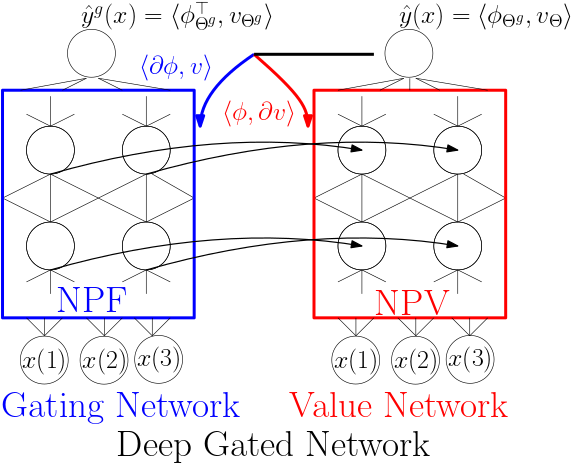
\includegraphics[scale=0.5]{figs/nntwin-blck.png}
}
\end{minipage}
\caption{}
\label{tb:dgn}
\end{table}
\end{comment}
\begin{assumption}\label{assmp:main}
(i) $\Theta_0\inrdnet$ is statistically independent of NPFs, (ii) $\Theta_0$ are sampled i.i.d from a distribution such that for any $\theta_0\in\Theta_0$,  we have $\E{\theta_0}=0$, and  $\E{\theta^2_0}=\sigma^2$, and $\E{\theta^4_0}={\sigma'}^2$.
\end{assumption}
\begin{theorem}[\textbf{Main Result}]\label{th:main} Under \Cref{assmp:main}, we have:\\
(i) $\E{K_0}=d\sigma^{2(d-1)} H_0=d\sigma^{2(d-1)} (x^\top x)\odot \lambda_0$.\\
(ii) In addition, if ${4d}/{w^2}<1$, then $Var\left[K_0\right]\leq O\left(d^2_{in}\sigma^{4(d-1)}\max\{d^2w^{2(d-2)+1}, d^3w^{2(d-2)}\}\right)$.
\end{theorem}
\begin{comment}
\begin{lemma}\label{lm:disentangle}[Disentanglement] Let $\nabla_{\Theta} v_t\in \R^{P\times d_{net}}$ be matrix whose entries are given by $\nabla_{\Theta} v_t (p,\theta)=\partial_{\theta}v_t(p),\forall p\in [P], \theta\in\Theta$, and let $I_P$ be the $P\times P$ identity matrix. Then, 
under \Cref{assmp:main}-(ii), it follows that $\E{\nabla_{\Theta}v_{\Theta_t})(\nabla_{\Theta}v_{\Theta_t})^\top }= d\sigma^{2(d-1)}I_{P}$.
\end{lemma}
\begin{comment}
\textbf{Proof of \Cref{th:main}-(i):} Let $\varphi_t=(\varphi_{p,t},p\in[P])\in \R^{d_{net}\times P}$ matrix, then since $K_t=\Psi^\top_t\Psi$, where $\Psi_t=\varphi_t \Phi_t$, we have $\E{K_t}=\E{\Phi^\top_t \varphi^\top_t \varphi_t \Phi_t}$. At initialisation, using the \Cref{assmp:main}-(i), we can pull out $\Phi^\top_t$ and $\Phi_t$ outside of the expectation to have \begin{align}\label{eq:pullout}\E{K_0}=\Phi^\top_0\E{ \varphi^\top_t \varphi_t }\Phi_0,\end{align} and from \Cref{lm:disentangle}, it follows that $\E{ \varphi^\top_t \varphi_t }=d\sigma^{2(d-1)}I$, and hence $\E{K_0}=d\sigma^{2(d-1)}\Phi^\top_0\Phi_0=d\sigma^{2(d-1)}H_0$.\\
\end{comment}
%This overlap is captured by $\lambda_t(s,s')$ which is the measure of overlap of the sub-networks that are active for both the inputs $x,x'\in\R^{d_{in}}$. Under. \Cref{assmp:main}, the inter-path interaction $\varphi^\top_t\varphi_t$ gets disentangled, result in the claim \Cref{th:main}-(i).\\
%However, in the later part of this section, we consider a special case, wherein, we give an explicit characterisation of the spectrum of $\E{K_0}$. Characterising $\lambda_0$ for the general case is left as future work.\\
\textbf{Role of Depth and Width:} Let us first look at the diagonal terms of $\lambda_0$. It is reasonable to assume that, owing to the symmetric nature of the weights, roughly $\mu=\frac{1}{2}$ fraction of the gates are \emph{on} every layer. Thus $\lambda_0(s,s)\approx (w/2)^{d-1}$. Now, due our choice of $\sigma=\sqrt{\frac{2}{w}}$, the diagonal entries will be close to $1$. We now turn our attention towards the non-diagonal entries of $\lambda_0$. Define $\tau(s,s',l)\stackrel{def}=\sum_{i=1}^w G_{x_s,t}(l,i)G_{x_{s'},t}(l,i)$ be the overlap of the active gates in layer $l$ for input examples $s,s'\in[n]$, and  let $\eta\stackrel{def}=\max_s\left(\max_{s',l} \frac{\tau(s,s',l)}{\tau(s,s,l)}\right)$ be the maximum overlap between gates of a layer (maximum taken over over input pairs $s,s'\in[n]$ and layers $l\in [d]$).  Then it follows that $\max_{s,s'\in [n]} \frac{\bar{\lambda}_{cross}(s,s')}{\bar{\lambda}_{self}(s)}\leq \eta^{d-1}$. Thus, the non-diagonal entries decay an exponential rate in comparison to the diagonal entries. The variance expression in \Cref{th:main}-$(ii)$ involves $d^2$ and $d^3$ terms, and hence for a fixed width as depth increases, the entries of $K_0$ deviates from $\E{K_0}$, and as a result the spectrum of $K_0$ degrades, thereby hurting training performance.\\
\subsection{Optimisation: General Case}
\textbf{Two random NTFs with identical random NPF:} As per \Cref{assmp:main}, the NPFs and NPVs are statistically independent at initialisation. In the case of random NPFs, this can be realised by first generating random NPFs corresponding to a random initialisation of weights (which is held in $\Theta'$), and  choosing $\Theta_0$ independent of $\Theta'$, and then updating $\Theta_t$ to learn the NPVs. In this case due to \Cref{th:main}, for infinitely large $w$, it follows that NTK is equal to NPK times a constant. Let us call this random NTK as RNTK-II (where `II' stands for \emph{independent initialisation}). On the contrary, we can generate the random NPFs with a random initialisation of weights $\Theta'$ and the let $\Theta_0=\Theta'$, and train $\Theta_t$ using GD. Here, NPFs and NPVs are not statistically independent at initialisation. We call the random NTK in this case as RNTK-DI (where `DI' stands for \emph{dependent initialisation}), which, in turn is given by $K_0=\Phi^\top_{\Theta_0}(\nabla_{\Theta} v_{\Theta_0})(\nabla_{\Theta} v_{\Theta_0})^\top \Phi_{\Theta_0}$. The `DI' case mimics the random NPFs and random NPVs of a DNN at random initialisation. Note that while the RNTK-DI and RNTK-II are different, their corresponding RNPK is identical, and the learning problem $\hat{y}_{\Theta}(x)=\ip{\phi_{x,\Theta'},v_{\Theta}}$ is the same. Thus, `II' and `DI' correspond to the same optimisation problem with fixed RNPFs, and the different initialisation only means different staring points for the GD procedure.  We also observe in our experiments that both II and DI cases yield same generalisation performance. 
\begin{comment}
\FloatBarrier
\begin{figure}[h]
%\begin{minipage}{0.78\columnwidth}
\resizebox{\columnwidth}{!}{
\begin{tabular}{ccc}
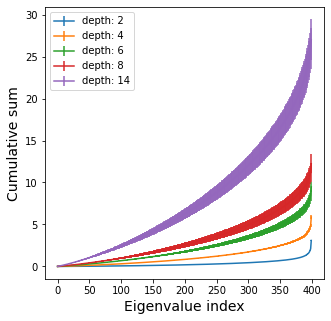
\includegraphics[scale=0.4]{figs/GaLU-ecdf.png}
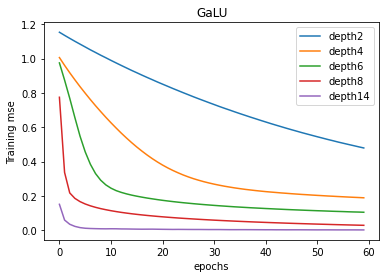
\includegraphics[scale=0.4]{figs/GaLU.png}
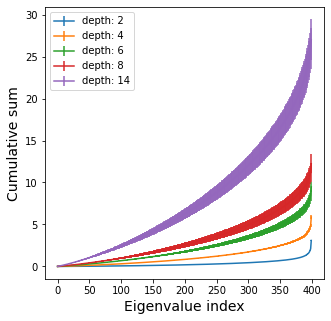
\includegraphics[scale=0.4]{figs/GaLU-ecdf.png}
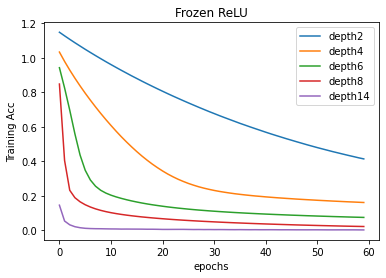
\includegraphics[scale=0.4]{figs/Frozen-ReLU.png}
%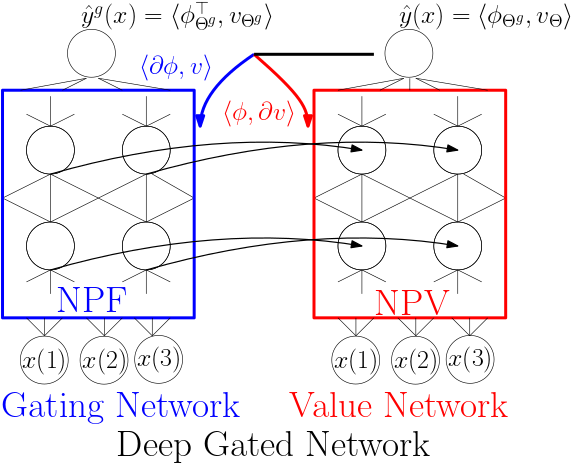
\includegraphics[scale=0.5]{figs/nntwin-blck.png}
%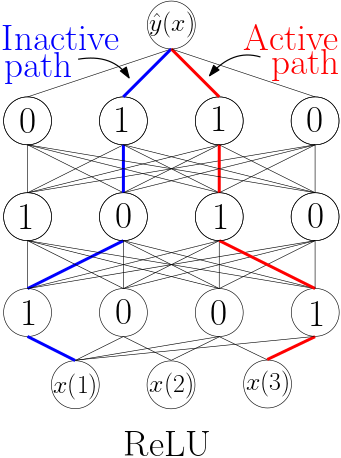
\includegraphics[scale=0.5]{figs/nn.png}
%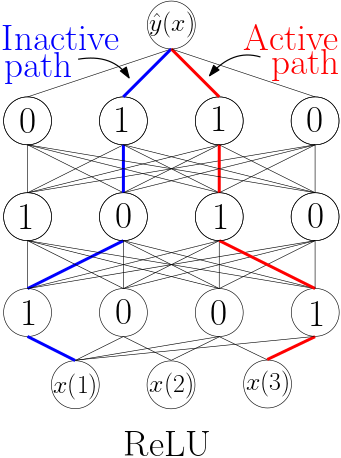
\includegraphics[scale=0.5]{figs/nn.png}
\end{tabular}
}
%\end{minipage}
%\begin{minipage}{0.18\columnwidth}
%\resizebox{\columnwidth}{!}{
%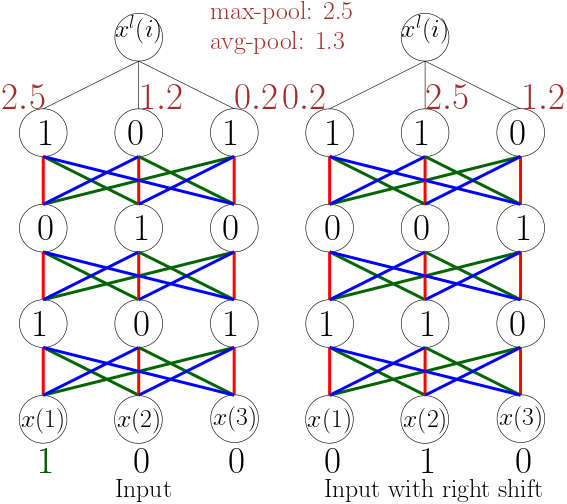
\includegraphics[scale=0.5]{figs/nnconv.png}
%}
%\end{minipage}
\caption{NPK}
\label{fig:opti}
\end{figure}
\end{comment}
